\section{流式数据更新}
\label{sec7:dynamic}

	区间森林算法RFS扩展了已有的核密度估计算法,在不额外增加时间复杂度的情况下扩展了带时间窗口的查询。然而,构造出来的区间森林索引是固定不变的,因此需要载入全部数据并确定整体索引结构后才可以进行构建和查询,无法支持动态插入。

	考虑到任意的动态插入问题比较复杂,我们考虑一个弱化的,但在现实生活中同样广泛的场景,即流式插入。流数据是一系列按照时间排序后的数据,需要将他们动态地依次插入索引中。流数据保证只会在数据末端插入。

	为了支持流数据的插入操作,我们需要将静态的索引改造成动态的索引。因此,我们提出了动态区间森林法(Dynamic Range Tree Solution,DRFS),其中每一个节点不再根据数据点的下标确定区间范围,而是直接根据边上的距离确定区间范围。

\subsection{动态区间森林法}

	DRFS算法的关键是将区间树和区间森林扩展成动态索引。和RFS算法类似,在DRFS算法中,动态区间树的每一个树节点 $u$ 同样会维护一个区间 $R(u)$。对于根节点来说,它会维护整条边上的数据,即 $R(root) = [0, d(v_c, v_d)]$。接着,每个树节点的左右孩子分别会维护一半的区间(而不是一半的数据):假设$R(u) = [l, r]$,那么左孩子的区间为$R(lc(u)) = [l, (l + r) / 2]$,右孩子的区间为$R(rc(u)) = [(l + r) / 2 + \delta, r]$。注意这里的$\delta$是一个无穷小量,用于避免区分两个区间。在这种顶一下,无需初始数据也可直接在原图上初步建立索引。

	图~\ref{fig:DRFS_1}展示了一个动态区间森林的例子,其中$\{o_1\}, \{o_2\}, \{o_3, o_4\}$分别落在第一、第三、第四个四分之一区间。区间森林上的查询(算法~\ref{algo:RFQ})和构造(算法~\ref{algo:RFC})同样适用于这个结构,只需要修改对应的区间$R(u)$即可。

\begin{figure}[h]\centering
	\scalebox{0.5}[0.5]{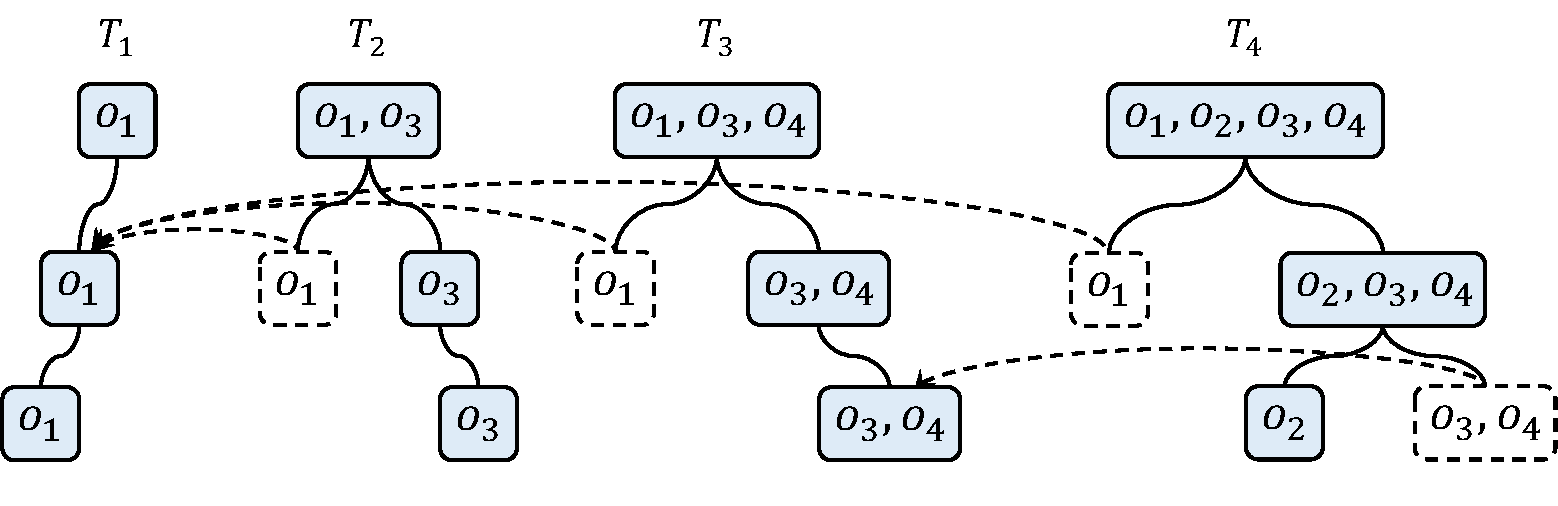
\includegraphics{./figures/DRFS_1.pdf}}
	\caption{一个动态区间森林的例子。现在区间森林节点的区间是根据边的实际距离而不是节点下标划分的。}
	\label{fig:DRFS_1}
\end{figure}

	DRFS算法并不是一个精确算法。在图~\ref{fig:RFS1}中,静态区间树的每一个叶节点都仅包含一个数据点,因此RFS可以精确的判断带宽范围所在的位置,并且获取精确的聚合向量。然而在图~\ref{fig:DRFS_1}中,动态区间树的部分叶节点可能包含多个数据点(例如$\{o_3, o_4\}$)。如果该节点是部分覆盖的,此时却并没有更深的一层节点用于更精准的探查,无论是否返回聚合向量都会导致答案出现误差。

	为了尽可能减少这一问题所带来的影响,我们进一步提出了扩展操作,用于扩展动态区间森林的层数。例如在图~\ref{fig:DRFS_1}中,三层索引不足以精准区分所有数据点,那么扩展操作就可以扩展出第四层,并更新相关索引。在图~\ref{fig:DRFS_2}中,一个四层的索引就足够划分所有数据点,其中被新扩展出的第四层结构用灰色方框展示。

\begin{figure}[h!]\centering
	\scalebox{0.5}[0.5]{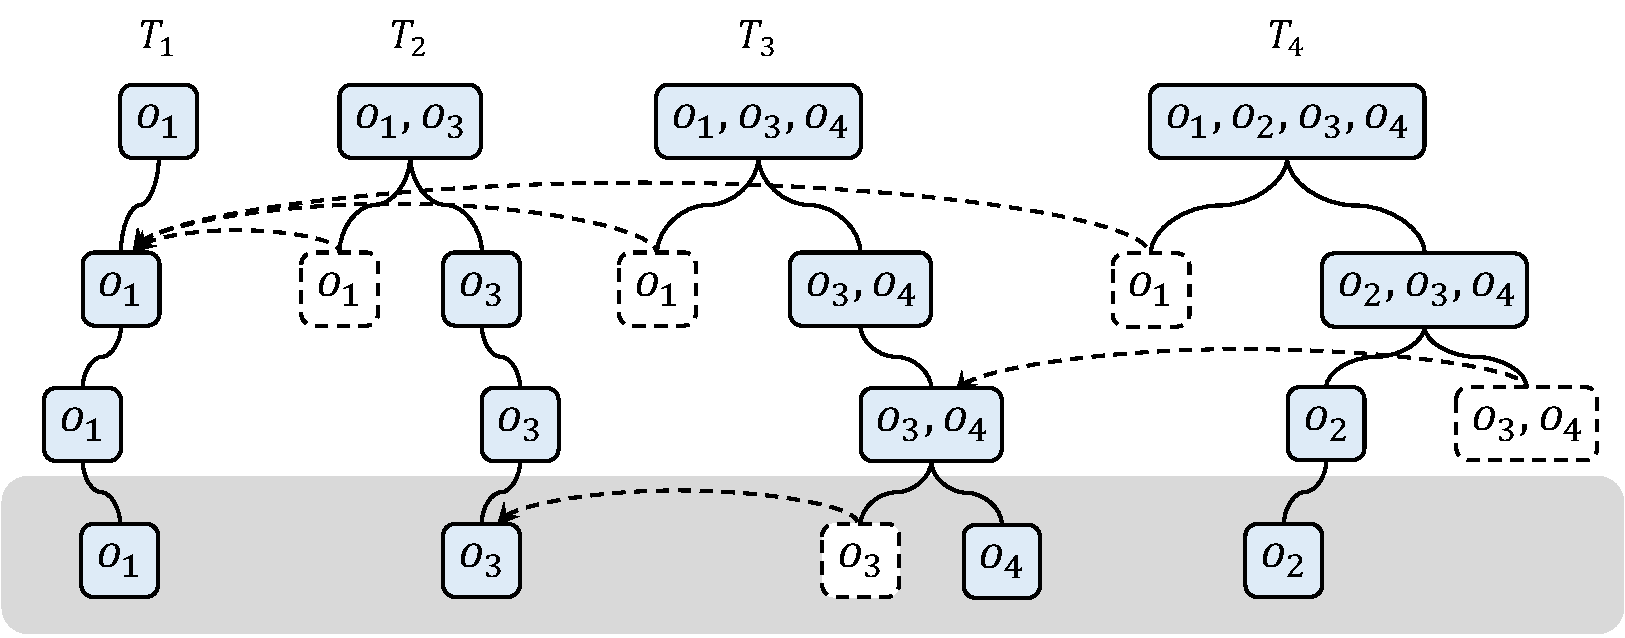
\includegraphics{./figures/DRFS_2.pdf}}
	\caption{一个动态区间森林扩展的例子。灰色矩形部分就是新扩展的一层。}
	\label{fig:DRFS_2}
\end{figure}

	这一扩展操作可以被视作是一个索引上的懒惰操作,在算法~\ref{algo:DRFS}中有相关的实现。具体来说,在初始构造或上一次扩展的同时,我们需要额外记录所有的叶节点$leaf_i$。当需要扩展新的一层时,可以直接对这些叶节点调用构造算法中的\textit{DualConstruct}函数。这就类似于将原来的构造函数中断,并在需要扩展时恢复。为了继续原来的构造步骤,只需要记录两个变量$o_i$和$u_l$,即所需要更新的数据点,以及前一棵区间树上的更新位置。

	\begin{algorithm}[t]
		\caption{Extension Operation}
		\label{algo:DRFS}
		\DontPrintSemicolon
		\KwIn{a range forest, event set $\{o_i\}$}
		\KwOut{a range forest with an extended layer}
		
		\For{each event $o_i$}{
	
			$u \leftarrow$ last updated node $leaf_i$
			
			call DualConstruct on $u$ to extend a new layer
	
			save new updated node $leaf_i$
		}
	
	\end{algorithm}

	因此,我们可以预先构造一个默认深度为$H$的动态区间森林,用户可以根据他们的精度和空间需求动态地调整深度参数 $H$。具体来说,深度越大,得到的结果精度也越高,但所占用的空间也会越大。并且,这种动态扩展的操作相比于直接构造并不会增加额外的时间开销,这就使得这种扩展操作更加灵活。

	\begin{lemma}
		DRFS算法的查询时间复杂度为$O(\vert E \vert (T_{sp} + L \cdot H))$,其中 $H$ 是森林的深度。无论是通过动态扩展构造,还是直接构造,索引的构造时间和空间复杂度均为$O(N \cdot H)$。
	\end{lemma}
	\begin{proof}
		根据引理~\ref{lemma:RFS_1},我们使用固定的树深度$H$代替原有的深度 $\log{n_e}$,其他部分的分析不变,因此时间复杂度为$O(\vert E \vert (T_{sp} + L \cdot H))$。
		
		构造一个深度为 $H$ 的区间森林需要 $O(n_e \cdot H)$ 的时间复杂度,使用算法~\ref{algo:DRFS} 扩展新的一层需要对每一个数据点所对应的区间树更新一次,即$O(n_e)$。因此,动态构造深度为 $H+1$ 的区间森林所需要的时间为 $O(n_e \cdot H) + O(n_e) = O(n_e \cdot (H+1))$,这和直接构造深度为 $H+1$ 的区间森林的时间复杂度是一样的。而索引的大小也是用固定的树深度$H$代替原有的深度 $\log{n_e}$,即$O(N \cdot H)$。
	\end{proof}


\subsection{动态区间森林结构的量化}

	真实场景下的应用对于索引大小是高度敏感的。只要精度在可以接受的范围内,一个相对较小的索引会更受欢迎。因此,通过对索引进行量化可以在保证查询精度尽可能保持不变的情况下减少索引的大小。
	
	由于动态区间森林的深度可以自由扩展新的层数以增大 $H$,或隐藏一些更深的层以减少 $H$,且而不会带来额外的开销,对高度 $H$ 进行量化是一个有效的手段。
	
	注意到在实际的运行过程中,大部分查询无需到达最深一层即会出现全覆盖或不覆盖的情况,此时即提前返回结果;另一方面,即使某次查询需要达到叶节点才能精确计算,提前结束查询所带来的误差并不会很大。因此,一个相对较小的量化高度$H$就可以快速产生一个相对比较精确的结果。

	量化的效果直接由量化高度$H$决定。减少$H$可以显著减少时间和空间消耗。作为交换,叶节点将包含更多事件,从而可能导致更多部分覆盖的情况。在我们的实验中,与精确结果相比,即使$H=2$也能达到超过90\$的精度,并且成本仅为原始数据内存的$2^{H}=4$倍,这揭示了量化的高缩放能力。

